% \newpage
% \begin{figure}
%     \centering
%     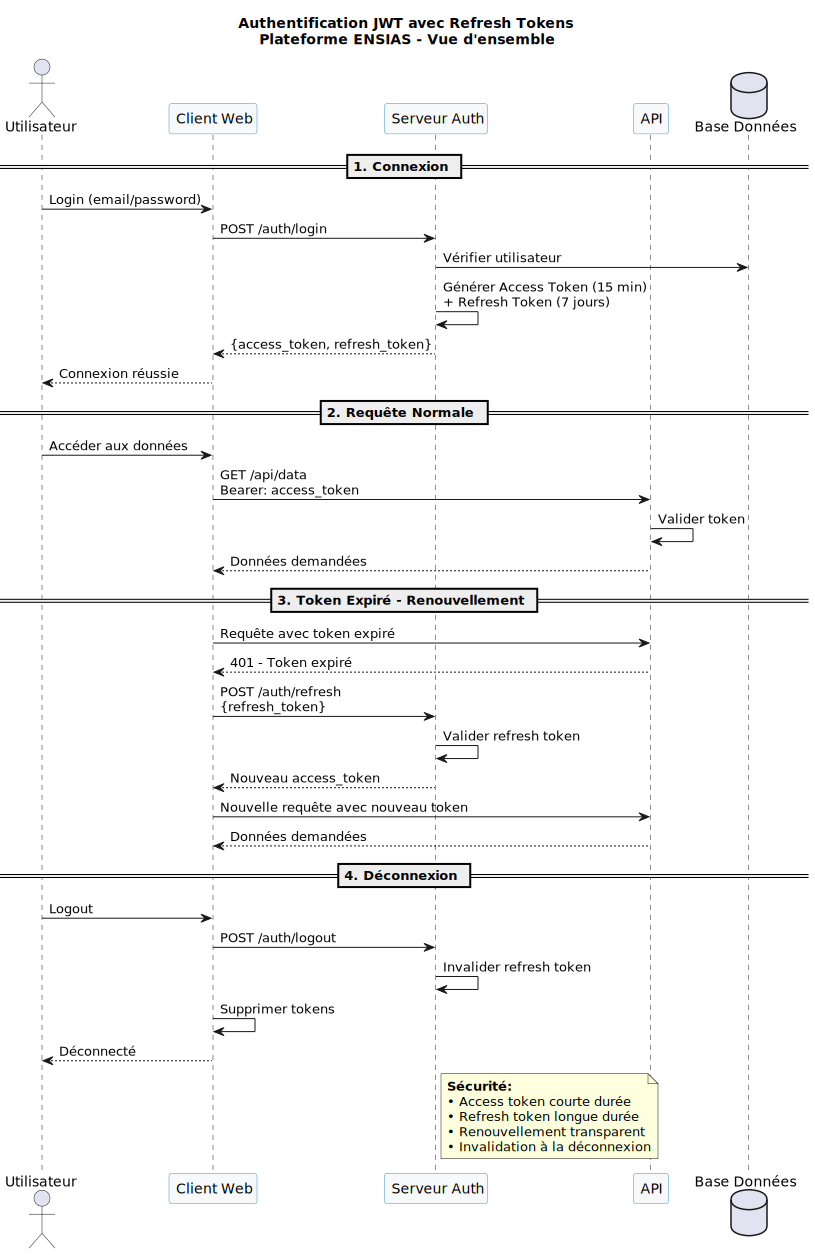
\includegraphics[width=0.5\linewidth]{diagrams/sequence_jwt.svg}
%     \caption{jwt sequence}
%     \label{fig:enter-label}
% \end{figure}

\item \textbf{Spring Boot :} Pour le développement de la partie backend de l'application. Ce framework Java basé sur Spring simplifie grandement la création d'applications robustes, performantes et autonomes. Il facilitera la mise en place rapide d'API RESTful, la gestion de la sécurité (par exemple avec Spring Security) et l'interaction avec la base de données (via Spring Data JPA).

\item \textbf{ReactJS :} Pour la construction de l'interface utilisateur (frontend). Cette bibliothèque JavaScript, maintenue par Facebook, permet de créer des interfaces utilisateur dynamiques et réactives basées sur une architecture de composants. Elle nous aidera à développer une expérience utilisateur moderne et attrayante, conformément aux objectifs du projet.

\item \textbf{PostgreSQL :} Notre système de gestion de base de données relationnelle (SGBDR). PostgreSQL est reconnu pour sa robustesse, sa conformité SQL avancée et ses fonctionnalités d'extensibilité. Il sera utilisé pour stocker et gérer toutes les données de l'application, telles que les informations sur les départements, les professeurs, les formations, les modules, etc., en respectant le modèle entité-relation conçu.

\item \textbf{Docker :} Pour la conteneurisation de notre application. Docker nous permettra d'empaqueter notre application (backend Spring Boot, frontend React servi par un serveur web léger comme Nginx, et potentiellement la base de données PostgreSQL pour l'environnement de développement/test) et ses dépendances dans des conteneurs isolés. Cela garantit la cohérence des environnements entre le développement, les tests et la production, et simplifie grandement le processus de déploiement.

\item \textbf{Oracle Cloud Infrastructure (OCI) / ou autre plateforme Cloud :} Bien que vous ayez mentionné OCI dans la liste des outils, cela se réfère généralement à l'infrastructure d'hébergement. Si OCI est votre cible de déploiement, Docker facilitera le déploiement des conteneurs sur les services de calcul d'OCI (comme Compute Instances ou Oracle Kubernetes Engine - OKE). Si "OCI" se référait à une technologie spécifique liée à Docker (comme Open Container Initiative), alors Docker lui-même est la technologie principale que vous utiliserez pour les conteneurs. Nous utiliserons une plateforme cloud (potentiellement OCI) pour héberger les différents services conteneurisés et rendre l'application accessible.

\item \textbf{Git (et une plateforme comme GitHub/GitLab) :} Pour la gestion de version du code source. Essentiel pour le travail collaboratif, le suivi des modifications, la gestion des branches pour les différentes fonctionnalités et la facilitation de l'intégration continue.